%!TEX root=main.tex

\chapter{Stateful Pipeline}

% Difference between stateless/stateful stage
As defined by the OpenFlow specification, a packet entering an OpenFlow switch is processed through a pipeline comprised of a set of linked flow tables that provide matching, forwarding, and packet modification. We indicate with the term \emph{stateless stage} the processing operated by a single stateless OpenFlow's flow table. Conversely, we define as \emph{stateful stage} (Figure~\ref{f:stateful-stage}) a logical stage comprising a state table and and a flow table, and implementing our abstraction.

\begin{figure}[h]
	\centering
	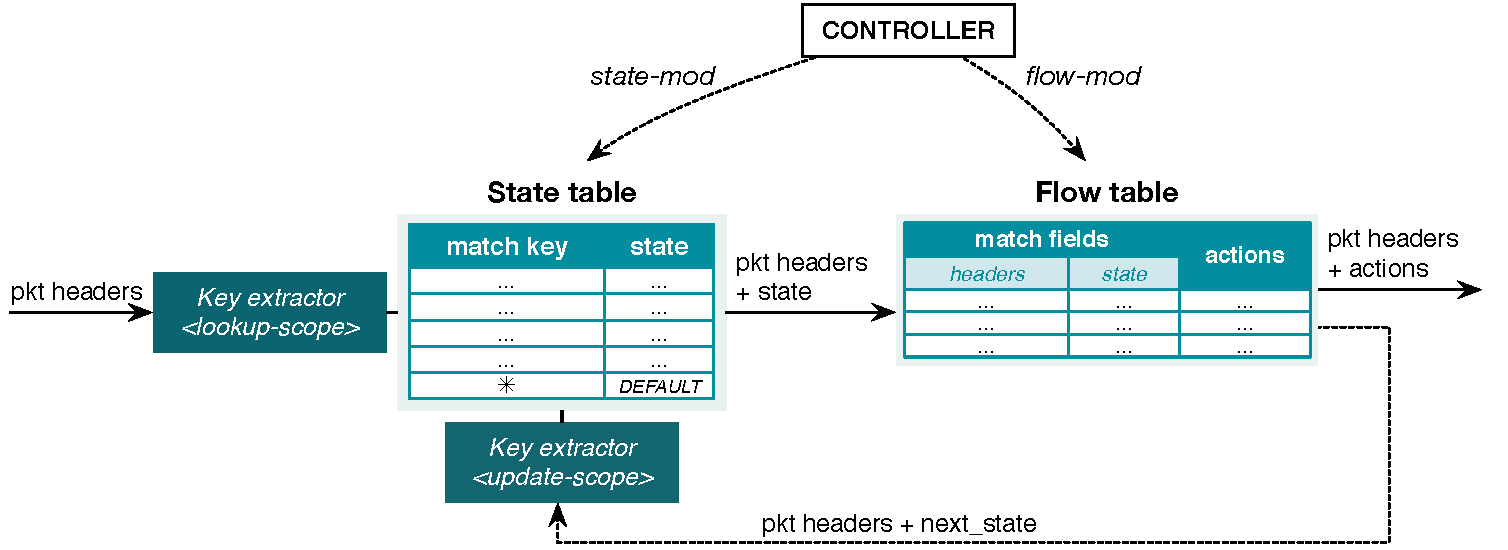
\includegraphics[width=\textwidth]{stateful-stage-arch}
	\caption{Architecture of an OpenState stateful stage}
	\label{f:stateful-stage}
\end{figure}

When a packet enters a stateful stage, it is first processed by a \emph{key extractor} which produces a string of bits representing the key to be used to match a row in the state table. The key is derived by concatenating the header fields defined in the \emph{lookup-scope}. The matched state label is appended to the packet headers as an additional header field. In case of a table-miss (the key is not matched) then a \emph{DEFAULT} state will be appended to the packet headers. If the header fields specified by the lookup-scope are not found (e.g. extracting the IP source address when the Ethernet type is not IP), a special state value \emph{NULL} is returned. By exiting the state table, packet headers along with the returned state label are matched in the flow table.

The flow table is extended by adding support to a new ``state'' virtual header field to be used to match packets along with classic header fields (MPLS, IP, TCP, etc.). We say this header is virtual because it is not really appended to the packet header and it is valid only for current processing trough the flow table of the stateful stage. Moreover a new set-state action is introduced to allow to update the state value for a given flow in a given stateful stage. The set-state action can be called as any other OpenFlow action.

\comment{Carmelo}{Is it correct to say that state labels are valid only inside the stateful stage that produced them? In other words, can I match on multiple state labels provided by different stateful stages?}

By default all the flow tables in the switch are intended as stateless stages, the controller can then enable stateful processing for one or more stages by sending a special control message to the switch and by configuring the key extractors (lookup-scope and update-scope) associated with the state table. Similarly to flow tables, new modification message called \emph{state-mod} has been defined to allow the controller to configure the state entries and key extractors.


\todo{Carmelo}{
	\begin{itemize}
		\item Global-states introduction
	\end{itemize}
}


%A new switch capability has been defined in order to support all the OpenState functionalities, namely flow-states and global-states. A new state modify message called \emph{state-mod} has been defined to allow the controller to configure the state entries and key extractors. Finally two new actions \textbf{set-state} and \textbf{set-flags} have been defined in order to respectively implement and configure the XFSM state transitions in the flow table and set the global states.